% Gemini theme
% https://github.com/anishathalye/gemini

\documentclass[final]{beamer}

% ====================
% Packages
% ====================

\usepackage[T1]{fontenc}
\usepackage{lmodern}
% Dimensions: 4'-by-3' in cm
\usepackage[size=custom,width=121.92,height=91.44,scale=1.0]{beamerposter}
\usetheme{gemini}
\usecolortheme{labsix}
\usepackage{graphicx}
\usepackage{booktabs}
\usepackage{tikz}
\usepackage{pgfplots}
\usepackage{multicol}
\usepackage[numbers]{natbib}
\usepackage{import}

% ====================
% Lengths
% ====================

% If you have N columns, choose \sepwidth and \colwidth such that
% (N+1)*\sepwidth + N*\colwidth = \paperwidth
\newlength{\sepwidth}
\newlength{\colwidth}
\setlength{\sepwidth}{0.025\paperwidth}
\setlength{\colwidth}{0.3\paperwidth}

\newcommand{\separatorcolumn}{\begin{column}{\sepwidth}\end{column}}

\title{The Sun at Scale: Interactive Analysis of SDO Data on HPC Platforms with Dask}

\author{Will Barnes \inst{1}\textsuperscript{,}\inst{2}\textsuperscript{,}\inst{3}\textsuperscript{\inst{\dagger}} \and
        Mark Cheung \inst{2} \and
        Monica Bobra \inst{3} \and
        Arthur Amezcua \inst{3} \and
        Herbert Yeung \inst{4}\textsuperscript{,}\inst{5} \and
        Stuart Mumford \inst{6}
}

\institute[]{
  \inst{1} Bay Area Environmental Research Institute \samelineand
  \inst{2} Lockheed Martin Solar and Astrophysics Laboratory \samelineand
  \inst{3} W. W. Hansen Experimental Physics Laboratory, Stanford University \and
  \inst{4} Arctic Slope Regional Corporation \samelineand
  \inst{5} NASA Ames Research Center \samelineand
  \inst{6} University of Sheffield \samelineand
  \inst{\dagger} Visiting Postdoctoral Scholar
}

\footercontent{
  \href{https://gitlab.com/wtbarnes/aia-on-pleiades}{gitlab.com/wtbarnes/aia-on-pleiades} \hfill
  AGU Fall Meeting 2019 --- San Francisco, CA USA --- 12 December 2019 \hfill
  \href{mailto:barnes@baeri.org}{barnes@baeri.org}
}

\begin{document}

% Logos
% LMSAL logo goes here
\addtobeamertemplate{headline}{} 
{
    \begin{tikzpicture}[remember picture,overlay] 
      \node [anchor=north west, inner sep=3cm] at ([xshift=1.4cm,yshift=1.3cm]current page.north west)     {\includegraphics[height=8cm]{../../logos/SU_Seal_Red.png}};
    \end{tikzpicture} 
}
\addtobeamertemplate{headline}{} 
{
    \begin{tikzpicture}[remember picture,overlay] 
      \node [anchor=north east, inner sep=3cm] at ([xshift=-8cm,yshift=1.3cm]current page.north east)     {
\includegraphics[height=8cm]{../../logos/sunpy_powered_logo.png}}; 
    \end{tikzpicture} 
}
\addtobeamertemplate{headline}{} 
{
    \begin{tikzpicture}[remember picture,overlay] 
      \node [anchor=north east, inner sep=3cm] at ([xshift=2cm,yshift=1.3cm]current page.north east)     {\includegraphics[height=8cm]{../../logos/agu_centennial.png}}; 
    \end{tikzpicture} 
}


\begin{frame}[t]
\begin{columns}[t]
\separatorcolumn

\begin{column}{\colwidth}

  \begin{block}{The Solar Dynamics Observatory}
    \begin{columns}
      \begin{column}{0.6667\columnwidth}
        A picture of the Sun as captured by SDO

        Followed by some facts about SDO/AIA and data products

        Make sure to emphasize the problem we are trying to solve!
      \end{column}
      \begin{column}{0.333\columnwidth}
        \begin{figure}
          \centering
          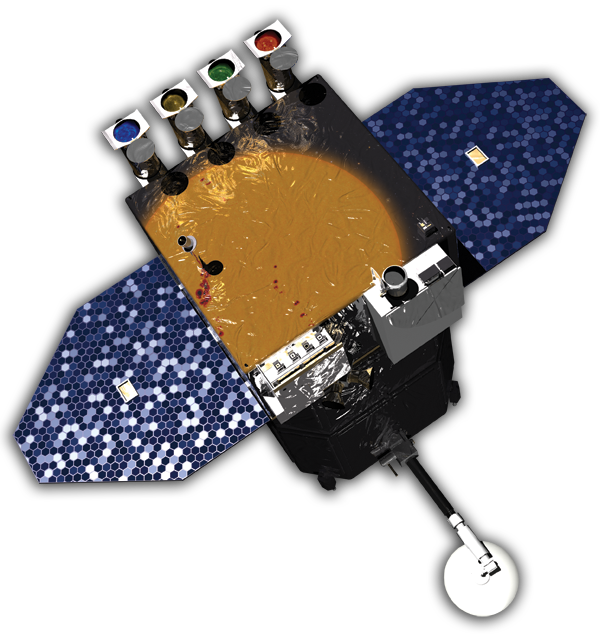
\includegraphics[width=\columnwidth]{figures/sdo.png}
        \end{figure}
      \end{column}
    \end{columns}

  \end{block}

  \begin{block}{An Interactive and Scalable Python Workflow}

    Diagrams of old workflow

    \begin{figure}
      \centering
      \def\svgwidth{0.7\columnwidth}
      \import{figures/}{old_workflow.pdf_tex}
      %\resizebox{0.65\columnwidth}{!}{\import{figures/}{old_workflow.pdf_tex}}
    \end{figure}

    Diagram of new workflow

    \begin{figure}
      \centering
      \def\svgwidth{0.8\columnwidth}
      \import{figures/}{new_workflow.pdf_tex}
      %\resizebox{0.65\columnwidth}{!}{\import{figures/}{old_workflow.pdf_tex}}
    \end{figure}

    Discuss each and why new one is better (briefly)


  \end{block}

  \begin{block}{Current Infrastructure}

    Describe what we've done so far

    Data moved from JSOC to Ames (see slides from Art)

    Query data using drms module \citet{glogowski_drms_2019}

    Jupyter notebooks running on Pleiades

    Emphasize use of Python

    Make case for Merope as a good platform for these types of workflows

  \end{block}

\end{column}

\separatorcolumn

\begin{column}{\colwidth}

  \begin{block}{Creating Level 1.5 Data Cubes}

    Universal need for aligned (i.e. de-rotated) level 1.5 data cubes

    Describe why this is important, what level 1.5 means

    Easily parallelized, why this is important (speed)

    Advantages of NDCube and Dask

    Store as Zarr for efficient, cloud-ready access

    Show Dask layout glyph, NDCube data model

    Estimate of how long it would take to process the current data volume from level 1 to level 1.5

  \end{block}

  \begin{block}{Example: Global EUV Waves}

    Why is this important, e.g. \citet{liu_truly_2018}

    Describe analysis pipeline, including gathering data

    Show plot of log running ratio

  \end{block}

  \begin{block}{Example: Time Lag Analysis}

    How can time lag analysis be used to understand coronal heating \citet{viall_evidence_2012}

    Describe time lag mathematically \citet{barnes_understanding_2019}

    Show time lag map for a single channel pair

    Show scaling of time lag calculation with number of cores

  \end{block}

\end{column}

\separatorcolumn

\begin{column}{\colwidth}

  \begin{block}{Example: Automatic Detection of Sunspots}

    Describe STARA algorithm \citet{watson_modelling_2009}

    What we did, why would we want to do this

    How fast was it (compare to serial computation)

    Show sunspot count as function of time, butterfly diagram

  \end{block}

  \begin{block}{Example: Calculating SHARP Features}

    Describe SHARPs: what they are, why they are useful, e.g. \citet{bobra_helioseismic_2014}

    Justify why recalculating them is useful (i.e. ML)

    Comment on speed increase of calculating in parallel

    Plot one of them (e.g. total unsigned flux) as a function of time

  \end{block}

  \begin{block}{Conclusions and Future Work}

    What do these examples demonstrate?

    Recommendation: heliophysics needs a hosted computing platform for interactive data analysis!

    Other disciplines are already embracing this, e.g. LSST, JWST, Pangeo

    Adoption of Python is crucial to making this happen 

    Will become increasingly important as data volumes grow, e.g. DKIST

  \end{block}

  \begin{block}{References}
    \scriptsize

    We thank Wei Liu, Ignacio Ugarte-Urra, and Fraser Watson for their help in developing example use cases. We also thank Jeff Becker and Bob Ciotti for their assistance with the Pleiades HPC system. 

      \begin{multicols}{2}
        \bibliographystyle{aasjournal.bst}
        \bibliography{references.bib}
      \end{multicols}

  \end{block}

\end{column}

\separatorcolumn
\end{columns}
\end{frame}

\end{document}
